\documentclass{optica-article}

\journal{opticajournal} % for journals or Optica Open

\articletype{Research Article}

\usepackage{lineno}
\linenumbers % Turn off line numbering for Optica Open preprint submissions.

\begin{document}

\title{Mid-Infrared Hyperspectral Microscopy with Broadband 1-GHz Dual Optical Frequency Combs}

\section{Abstract}
% v1:
% Developing compact and robust systems that offer both high speed and wide bandwidth in the mid-infrared range is crucial for advancing vibrational spectroscopic imaging. In this study, we experimentally showcase the integration of broadband, high-repetition-rate dual-comb spectrometers (DCS) in the mid-infrared range with a scanning microscope. To illustrate this, we employ a set of 1-GHz mid-infrared frequency combs, demonstrating their capability for high-speed and broadband hyperspectral imaging. The system covers \mbox{1000 $\mathrm{cm^{-1}}$} at \mbox{$\mathrm{\lambda_c=3.4 \; \mu m}$} with 13.47 kHz spectra acquisition rate and \mbox{4 $\mathrm{\mu m}$} spatial resolution. Furthermore, we elucidate the trade-off between bandwidth and speed in DCS as it relates to microscopy. This provides a roadmap for the future advancement of high-repetition-rate DCS hyperspectral imaging.

% v2:
Mid-infrared microscopy is an important tool for biological analyses, allowing a direct probe of molecular bonds in their low energy landscape. In addition to the label-free extraction of spectroscopic information, the application of broadband sources can provide a third dimension of chemical specificity. However, to enable widespread deployment, mid-infrared microscopy platforms need to be compact and robust while offering high speed, broad bandwidth and high SNR. In this study, we experimentally showcase the integration of broadband, high-repetition-rate dual-comb spectrometers (DCS) in the mid-infrared range with a scanning microscope. To illustrate this, we employ a set of 1-GHz mid-infrared frequency combs, demonstrating their capability for high-speed and broadband hyperspectral imaging. The system covers 1000 $\mathrm{cm^{-1}}$ at $\mathrm{\lambda_c=3.4 \; \mu m}$ with 13.47 kHz spectra acquisition rate and 4 $\mathrm{\mu m}$ spatial resolution. Furthermore, we elucidate the trade-off between bandwidth and speed in DCS as it relates to microscopy. This provides a roadmap for the future advancement of high-repetition-rate DCS hyperspectral imaging.

% Recipe for a good abstract: 1. start with a broad statement (1-2 sentences) of the general importance/interest of the field. e.g. Even after xx years of developments, microscopy continues to be a field a scientific importance because of xx and yy. 2. Transition to what the outstanding problem in the field (I think this ties in with your original lead off sentence). 3. How does your work address/solve this problem. 4. Some details of your research and most important results (you already have this). 5. Conclude with a sentence or two of what your results will enable.

\section{Introduction}
% If we're trying to avoid the review paper feel, we could shorten or combine this paragraph on vibrational spectro-imaging at large with the next paragraph that motivates mid-infrared spectro-imaging.
Vibrational spectroscopy is a cornerstone technique for molecular characterization that provides detailed insights into molecular structures, interactions, and dynamics. At its core, it identifies the unique vibrational "fingerprints" of molecules, revealing their specific characteristics and behaviors. While this method provides deep insights into the molecular makeup, spectroscopic imaging has enhanced its scope. Spectroscopic imaging marries the depth of vibrational spectroscopy with spatial context, presenting a combined image where one can pinpoint not just which molecules are present but also their exact locations. This enhanced perspective is invaluable across diverse fields, from understanding material properties to probing biological systems, facilitating a richer and more precise understanding of intricate molecular landscapes.

Vibrational spectroscopy using mid-infrared light ($\sim$2 - 12 $\mathrm{\mu m}$) proves beneficial in bio-imaging because it provides label-free chemical contrast and can non-invasively identify the biomolecular composition of samples \cite{bakerUsingFourierTransform2014}. Tissues, cells, and other biological entities can be analyzed without external dyes or markers, preserving the sample's native state. This is essential in clinical applications, where assessing the safety and efficacy of external contrast agents can be challenging. Spectroscopic imaging can complement conventional diagnostic techniques as the sample remains undisturbed. While spectroscopic imaging offers invaluable chemical insights, its slow signal acquisition has hindered its widespread adoption in biomedical and clinical settings. The trade-off between speed and bandwidth in recent systems \cite{zhangDepthresolvedMidinfraredPhotothermal2016,koleDiscreteFrequencyInfrared2012,yehFastInfraredChemical2015}  based on mid-infrared laser sources can compromise its competitiveness against label-based fluorescence microscopy, the principal bio-imaging technology.

In this work, we utilize a set of recently developed 1-GHz mid-infrared frequency combs \cite{hoghooghiBroadband1GHzMidinfrared2022} to integrate a dual-comb spectrometer with a confocal microscope. We capitalize on the high repetition rate by fully filling the third Nyquist band (\mbox{2595 $\mathrm{cm^{-1}}$}--\mbox{3890 $\mathrm{cm^{-1}}$} at \mbox{$\Delta f_r=12.86 \; \text{kHz}$}). The system is among the fastest performers in the class of spectrometers covering over \mbox{1000 $\mathrm{cm^{-1}}$} with high spectral resolution in the mid-infrared.

The effort to push the barrier of spectral acquisition speed without compromising bandwidth is illustrated in \mbox{Fig. \ref{fig:bckgnd}} with a visual overview of significant developments in hyperspectral vibrational imaging over the last two decades. Experiments are mapped onto the two important metrics of spectra acquisition speed, which captures the rate at which spectra are gathered, and optical bandwidth, which captures the breadth of chemical content that can be observed. The two variables are plotted against each other since a significant difficulty lies in achieving both metrics simultaneously. For a better one-to-one comparison, the acquisition speeds listed for experiments that use focal plane arrays have been normalized to that of an analogous point scanning experiment.

% add qcl to the plot?, 
% and standard FTIR?

\begin{figure}[h]
    \centering
    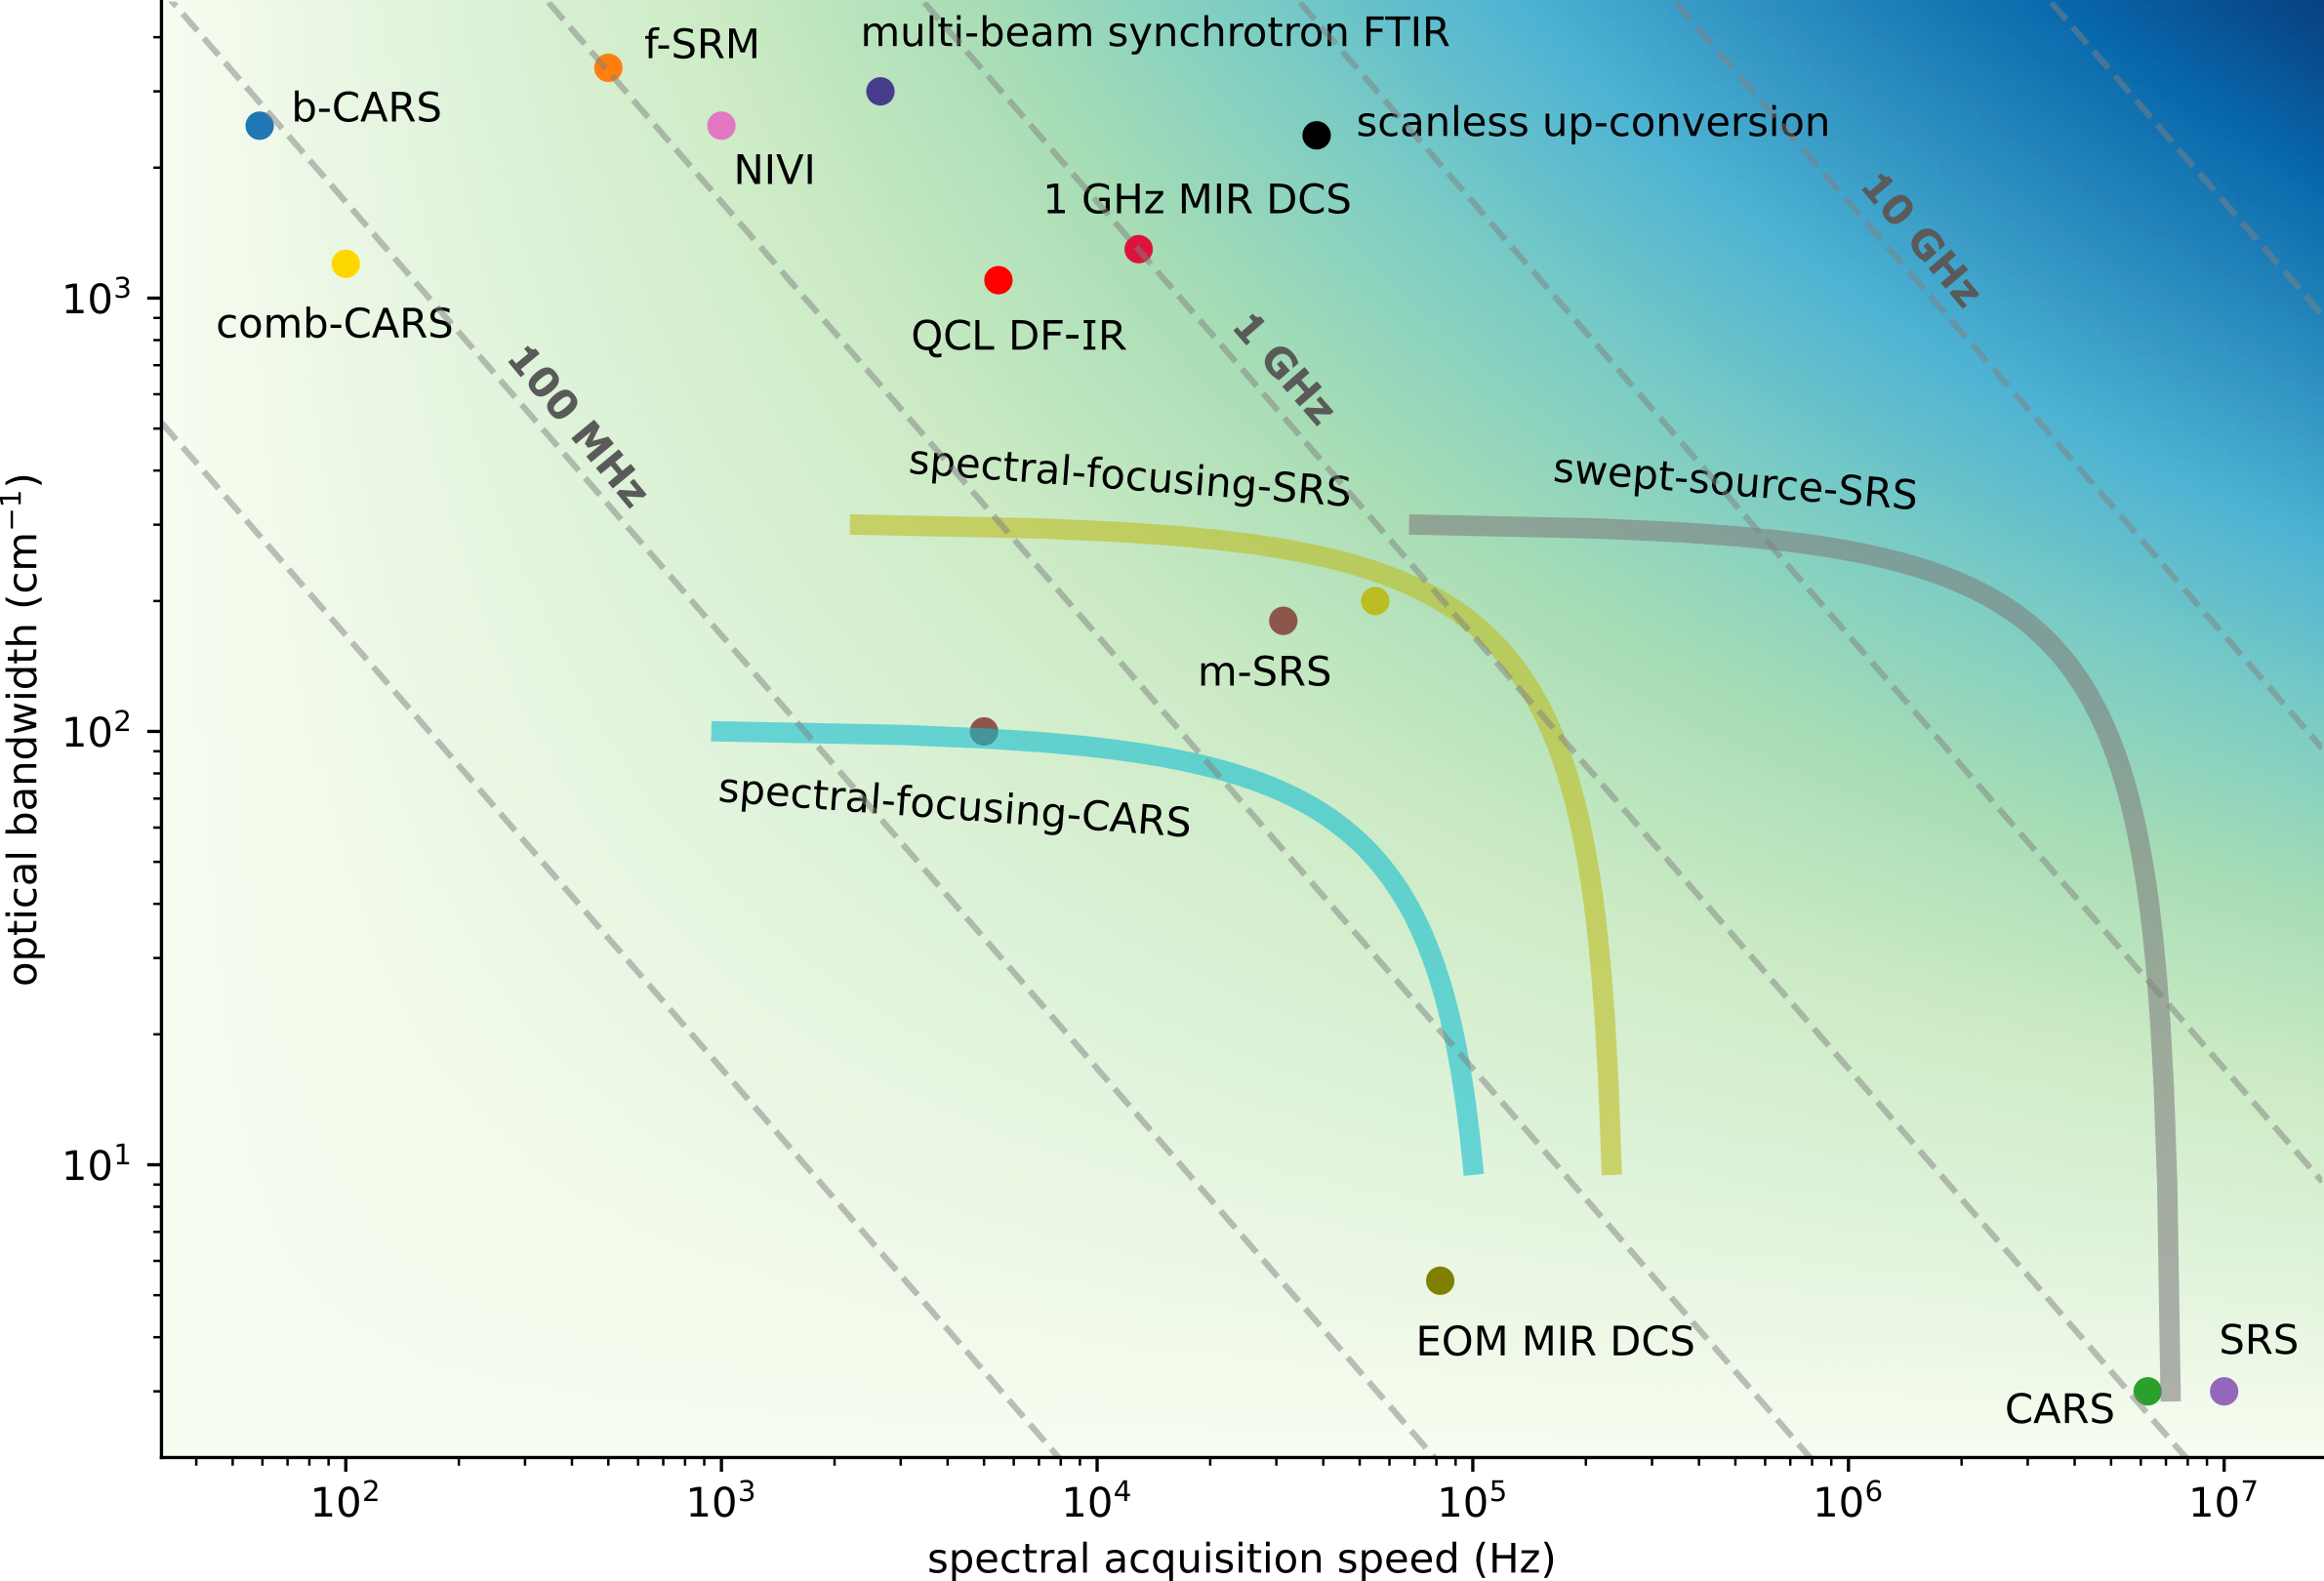
\includegraphics[width=\linewidth]{bckgnd_with_cm_v3.png}
    \caption{Performance map of mid-infrared hyperspectral imaging. Broadband CARS (b-CARS) \cite{keeSimpleApproachOnelaser2004}, femtosecond Stimulated Raman Microscopy (f-SRM) \cite{ploetzFemtosecondStimulatedRaman2007}, in-vivo video rate CARS \cite{evansChemicalImagingTissue2005}, in-vivo video rate SRS \cite{saarVideoRateMolecularImaging2010}, multiplexed SRS (m-SRS) \cite{fuQuantitativeChemicalImaging2012,liaoMicrosecondScaleVibrational2015}, nonlinear interferometric vibrational imaging (NIVI) \cite{chowdaryMolecularHistopathologySpectrally2010}, swept-source SRS \cite{ozekiHighspeedMolecularSpectral2012}, spectral-focusing SRS \cite{fuHyperspectralImagingStimulated2013}, spectral-focusing CARS \cite{dinapoliHyperspectralDifferentialCARS2014}, spectral-focusing SRS \cite{linMicrosecondFingerprintStimulated2021}, comb-CARS \cite{ideguchiCoherentRamanSpectroimaging2013}, multi-beam synchrotron FTIR \cite{nasseHighresolutionFouriertransformInfrared2011}, electro-optic modulator comb MIR DCS \cite{ullahkhanDirectHyperspectralDualcomb2020}, QCL discrete frequency infrared imaging (DF-IR) \cite{yehFastInfraredChemical2015}, scanless mid-infrared up-conversion imaging \cite{zhaoHighspeedScanlessEntire2023}}
    \label{fig:bckgnd}
\end{figure}

% The platform that claims one of the longest history in bio-imaging with many variations in design is coherent Raman spectro-imaging, where in-vivo video-rate speeds have been demonstrated in the mid-infrared \cite{evansChemicalImagingTissue2005, saarVideoRateMolecularImaging2010} using well-established near-infrared femtosecond oscillators. 

Coherent Raman spectro-imaging has achieved in-vivo video-rate speeds in the mid-infrared \cite{evansChemicalImagingTissue2005, saarVideoRateMolecularImaging2010} using well-established near-infrared femtosecond oscillators. Whereas initial demonstrations were over a narrow bandwidth (\mbox{$\sim$3 $\mathrm{cm^{-1}}$}), broad bandwidths at high acquisition speeds have been achieved using rapidly rotating polygonal mirror scanners \cite{tamamitsuUltrafastBroadbandFouriertransform2017, linMicrosecondFingerprintStimulated2021}. The stated metrics are possible with the strong Raman absorption cross-sections around \mbox{2900 $\mathrm{cm^{-1}}$}, which precludes Raman spectroscopy-based platforms from reaching the same performance in the fingerprint region at longer wavelengths. An important target is to achieve similar performance with direct mid-infrared illumination.

Fourier transform spectroscopy (FTS) and quantum cascade laser (QCL) based imaging are attractive due to their broad applicability across the mid to long wavelength infrared. The high absorption cross-sections can also alleviate the need for operation at powers close to sample-damage thresholds, a concern that is applicable to biological samples. In this category, FTS spectrometers coupled to broadband and bright sources such as synchrotron facilities have set the state of the art for the combination of spectral bandwidth and speed \cite{nasseHighresolutionFouriertransformInfrared2011}. The coupling of broadband synchrotron light into a microscope requires the active stabilization of a beam bundle. A widely accessible imaging method would benefit from having a table top setup. QCL lasers are attractive due to their direct emission in the mid-infrared and small footprint, although their performance is best leveraged in narrowband applications. Tunable QCL packages consisting of multiple QCL chips combined into one device \cite{yehFastInfraredChemical2015,goyalActiveHyperspectralImaging2014,zimmerleiterQCLbasedMidinfraredHyperspectral2021} can nominally reach broad spectral coverage, but further improvement is needed to reach noise figures comparable to platforms based on mode-locked lasers.

% insert zhao's paper here, i still need it to come last because i want to propose DCS as an alternative platform, not strictly a better one.
% you could use more QCL papers

% up conversion is not new, you should present it as one method, the pinnacle of which is below. take a look at the zotero folder i've made.

A popular alternative method to boost imaging speed in the mid-infrared is to employ up-conversion to shorter wavelengths in order to leverage low-cost near-infrared cameras, whose performance can significantly exceed mid-infrared focal plane arrays \cite{junaidVideorateMidinfraredHyperspectral2019,knezInfraredChemicalImaging2020,potmaRapidChemicallySelective2021}. A recent demonstration of this covered \mbox{$>$$1000 \; \mathrm{cm^{-1}}$} \cite{zhaoHighspeedScanlessEntire2023} in eight seconds. In this modality, a few cycle mid-infrared pulse is imaged from the sample plane onto a $\chi^{(2)}$ nonlinear crystal where it is overlapped with a long near-infrared pump pulse. The pump pulse's long picosecond duration causes the generated sum frequency light to encode the free-induction decay with few wavenumber resolution. Mapping the mid-infrared image to the near-infrared allows the use of a high-speed near-infrared hyperspectral camera. A few potential drawbacks is that the crystal thickness cannot exceed a few micron in order to be artifact free, and the frequency axis and spectra need to be calibrated and retrieved due to cross-phase modulation \cite{leeRemovingCrossphaseModulation2009}. This platform also carries a demand for very high pump pulse energies on the millijoule scale, requiring large regenerative amplifiers and a bulky apparatus.

% A recent demonstration of this with the broadest bandwidth and speed to date was able to cover

% The most recent Khan paper is a futher analysis of their previous work, particularly they go to very high frequency resolution which is a different direction than what you're discussing? They bring to light the QCL work though that I think we need to address ...

% something like: tunable QCL's consisting of multiple QCL chips can compensate the narrow spectral coverage, but without significant post-processing, so far struggle to reach noise figures comparable to light generated from mode-locked laser systems.

% Ideally, a compact and deployable imaging system could consider moving from the kilohertz solid state laser to well-developed fiber integrated light sources. 

The goal of a compact and deployable imaging system motivates parallel development of platforms seeded by well-developed fiber integrated light sources. Such oscillators are difficult to employ in already developed scanless imaging, however, due to the pulse energies of fiber amplifiers falling much below a millijoule, typically on the 1 - 10 nanojoule scale. 

In this work, we explore and apply high rep-rate dual-comb spectroscopy (DCS) to hyperspectral imaging. DCS has emerged as a powerful technique due to its combination of resolution, stability, and speed when compared to classical FTS \cite{coddingtonDualcombSpectroscopy2016}. In this modality, the interference of two frequency combs maps a Nyquist band from the optical domain down into the RF. One of the most important considerations in DCS is the direct trade-off between the frequency resolution/repetition rate $f_r$ and the size of the optical Nyquist window $\Delta \nu$:
% 
\begin{align}
    \Delta \nu = \frac{f_r^2}{2 \Delta f_r}
\end{align}
% 
where $\Delta f_r$ is the interferogram acquisition rate equal to the difference of the two laser rep-rates. The diagonal dashed lines in \mbox{Fig. \ref{fig:bckgnd}}., show the $f_r^2/2$ trade-off between resolvable bandwidth and acquisition speed in DCS for different $f_r$. Evidently, when broad absorption features allow for coarse resolution, the highest rep-rates are desired. However, in order to reach sufficient power per comb tooth, in practice the pulse energy required for nonlinear frequency down-conversion from the near-infrared sets an upper limit on the obtainable rep-rate. Shown in the upper right region of \mbox{Fig. \ref{fig:bckgnd}}, broadband hyperspectral imaging that is simultaneously high speed has poor representation from DCS platforms, largely because of the high rep-rates that would be required in order to compare to scanless methods. Whereas gigahertz mid-infrared frequency combs have already been demonstrated at rep-rates higher than a gigahertz \cite{kowligyMidinfraredFrequencyCombs2020} and even used for imaging \cite{ullahkhanDirectHyperspectralDualcomb2020,khanSubGHzOpticalResolution2023}, much of these are based on EOM generated combs which are difficult to generalize to cover broad bandwidths at sufficient power when considering collection through a microscope, and have been better applied to gas area monitoring. Here, we demonstrate broadband 1 GHz mid-infrared dual comb imaging based on a mode-locked laser platform.

% I think you say "repetition rate" too many times

However, pointing to the dashed line in the upper right corner of \mbox{Fig. \ref{fig:bckgnd}}, in order to achieve the ultimate goal of label-free broadband video-rate imaging, we note that the ideal DCS platform would operate with repetition rates of 10 GHz or higher. Such systems would likely require either high-power fiber amplifiers or a nanophotonic design capable of generating equivalent bandwidths in the mid-infrared with pump pulse energies around 100 pJ.

% Compared to previous work in dual-comb MIR imaging \cite{ullah_khan_direct_2020}, we show

% compared to previous work in dual-comb mir imaging \cite{khan...}, we show a significant improvement over...
% actually not really a one to one comparison, just mention their work instead?

% in this work we use a recently developed 1 GHz ... coupled to a confocal microscope ... the pixels are scanned continusouly, the imaging speed is limited by the laser repetition rate of ... kHz

% The EOM MIR DCS is actually at 18 GHz, but they use an FPA so they can't go as fast as the repetition rate allows them for each pixel at a time.

\section{Experiment and Results}

% you mentioned pulse energy difficulty before, maybe a brief but to the point statement of how this is achieved in this system

With long-term stability in mind, a single-branch intra-pulse difference frequency generation (DFG) design is used to generate frequency comb light in the mid-infrared. 
% 
% \begin{figure}[h]
%     \centering
%     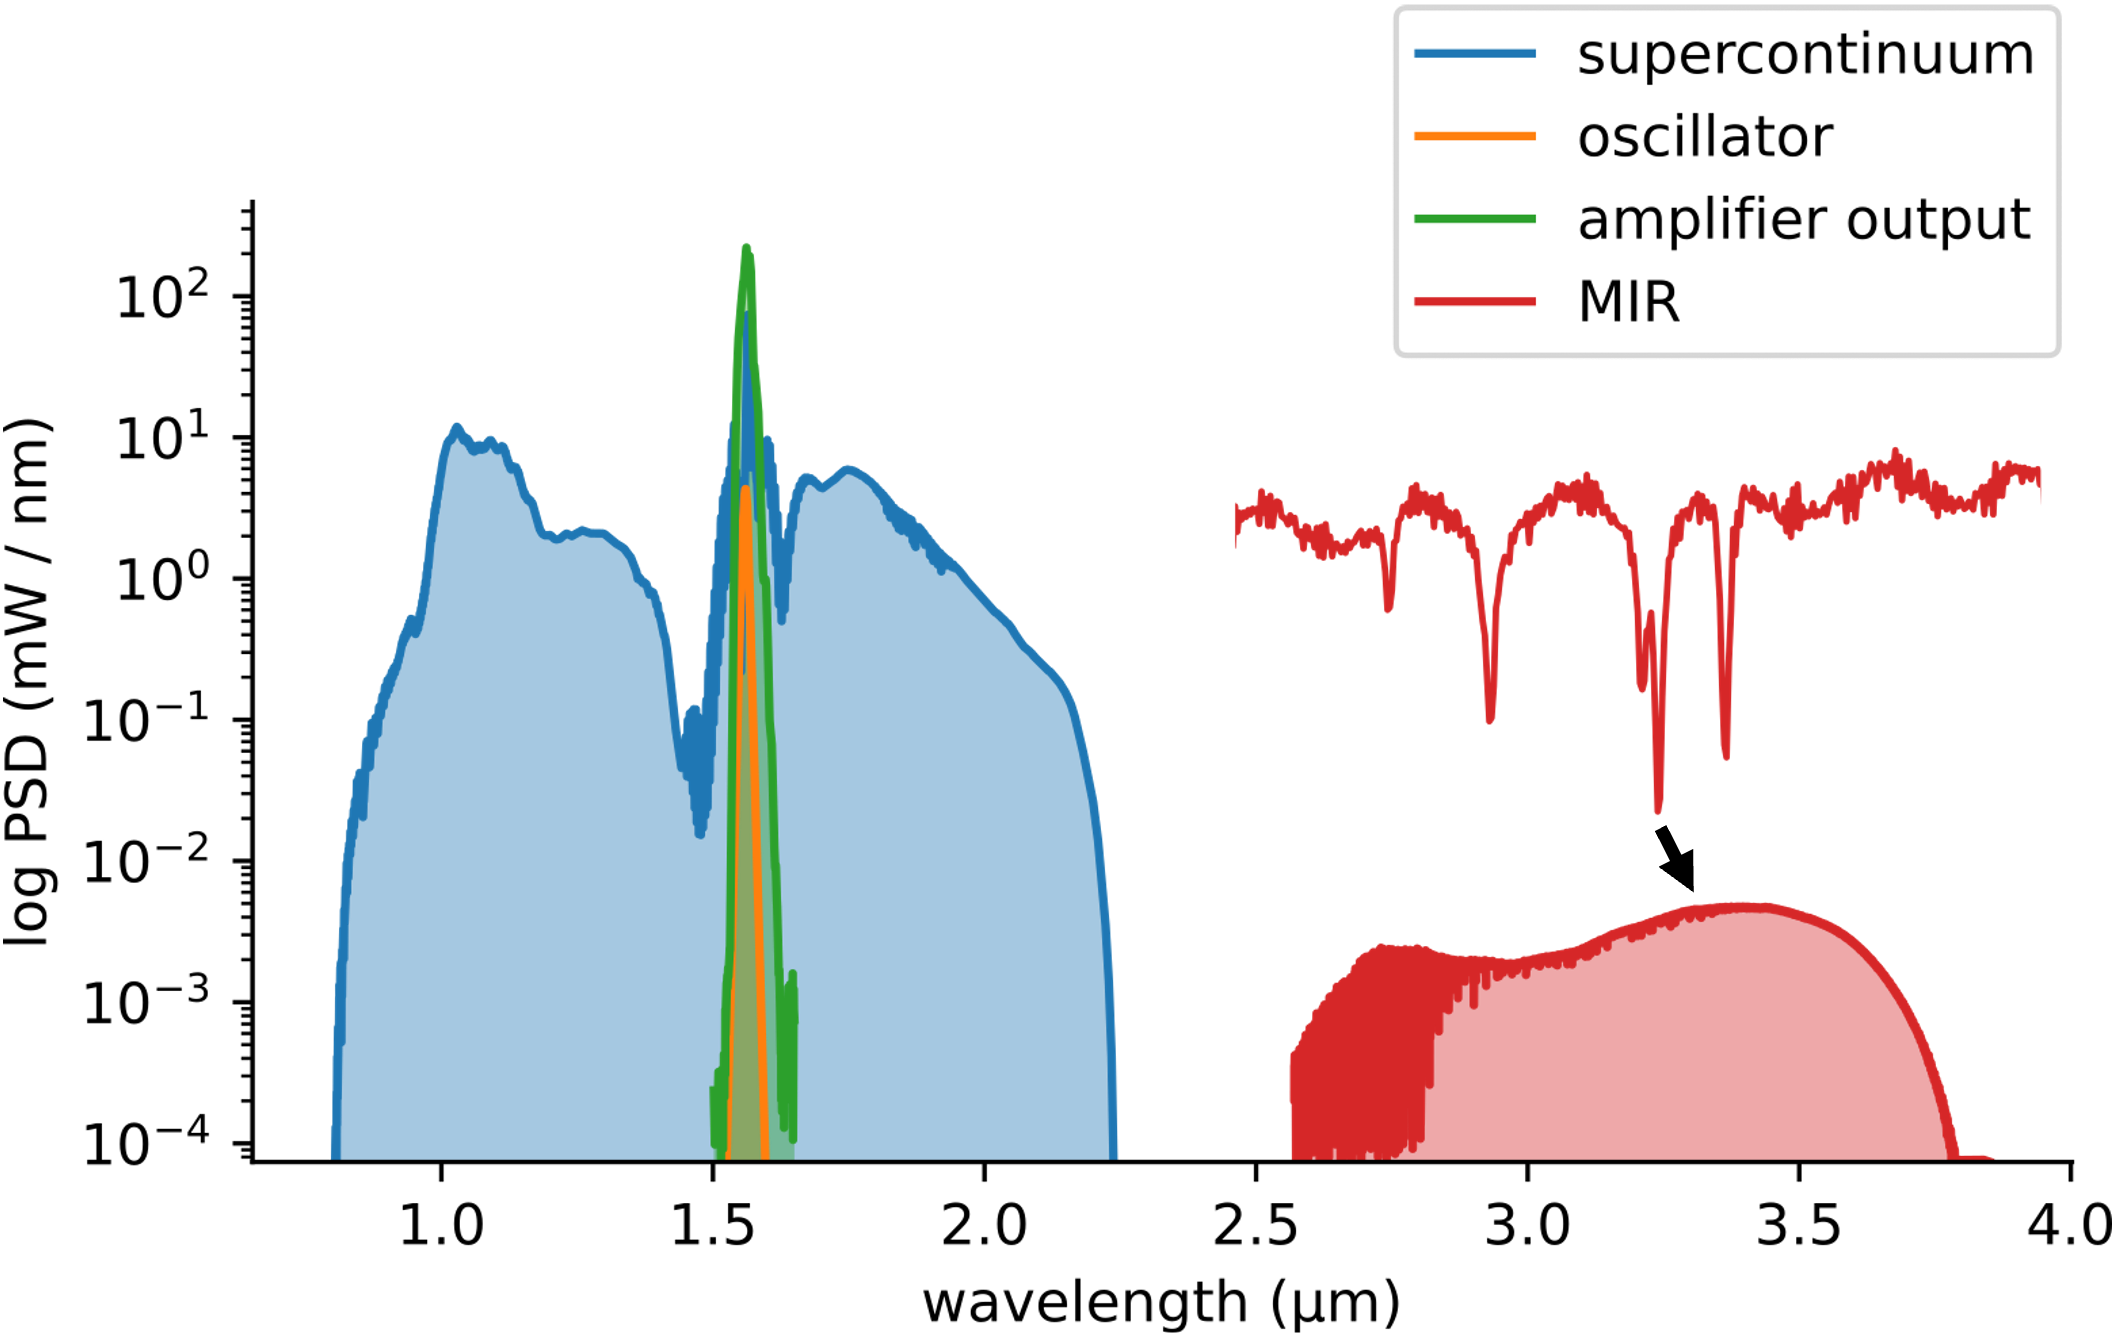
\includegraphics[width=\linewidth]{spectrum_in_setup.png}
%     \caption{1 GHz MIR Frequency Comb. The spectral evolution through successive stages of the system: oscillator $\rightarrow$ chirped-pulse amplifier $\rightarrow$ few-cycle supercontinuum generation $\rightarrow$ MIR frequency down conversion. The inset shows a zoom in of waterlines that are resolved when using the full 1 GHz frequency resolution.}
%     \label{fig:spectrum_in_setup}
% \end{figure}
%
Shown in \mbox{Fig. \ref{fig:setup}}, to compensate for the low conversion efficiency of the single-branch design, octave spanning few cycle NIR pulses generated via soliton self-compression in anomalous dispersion highly nonlinear fiber are used to drive the nonlinear frequency down conversion to the mid-infrared. Although coverage of the 6-13 $\mathrm{\mu m}$ wavelength region can be achieved for one laser system \cite{hoghooghiBroadband1GHzMidinfrared2022}, due to the lack of nonlinear crystals in this work more widely available lithium niobate is used to cover the 3 - 5 $\mathrm{\mu m}$ wavelength window.

\begin{figure}[h]
    \centering
    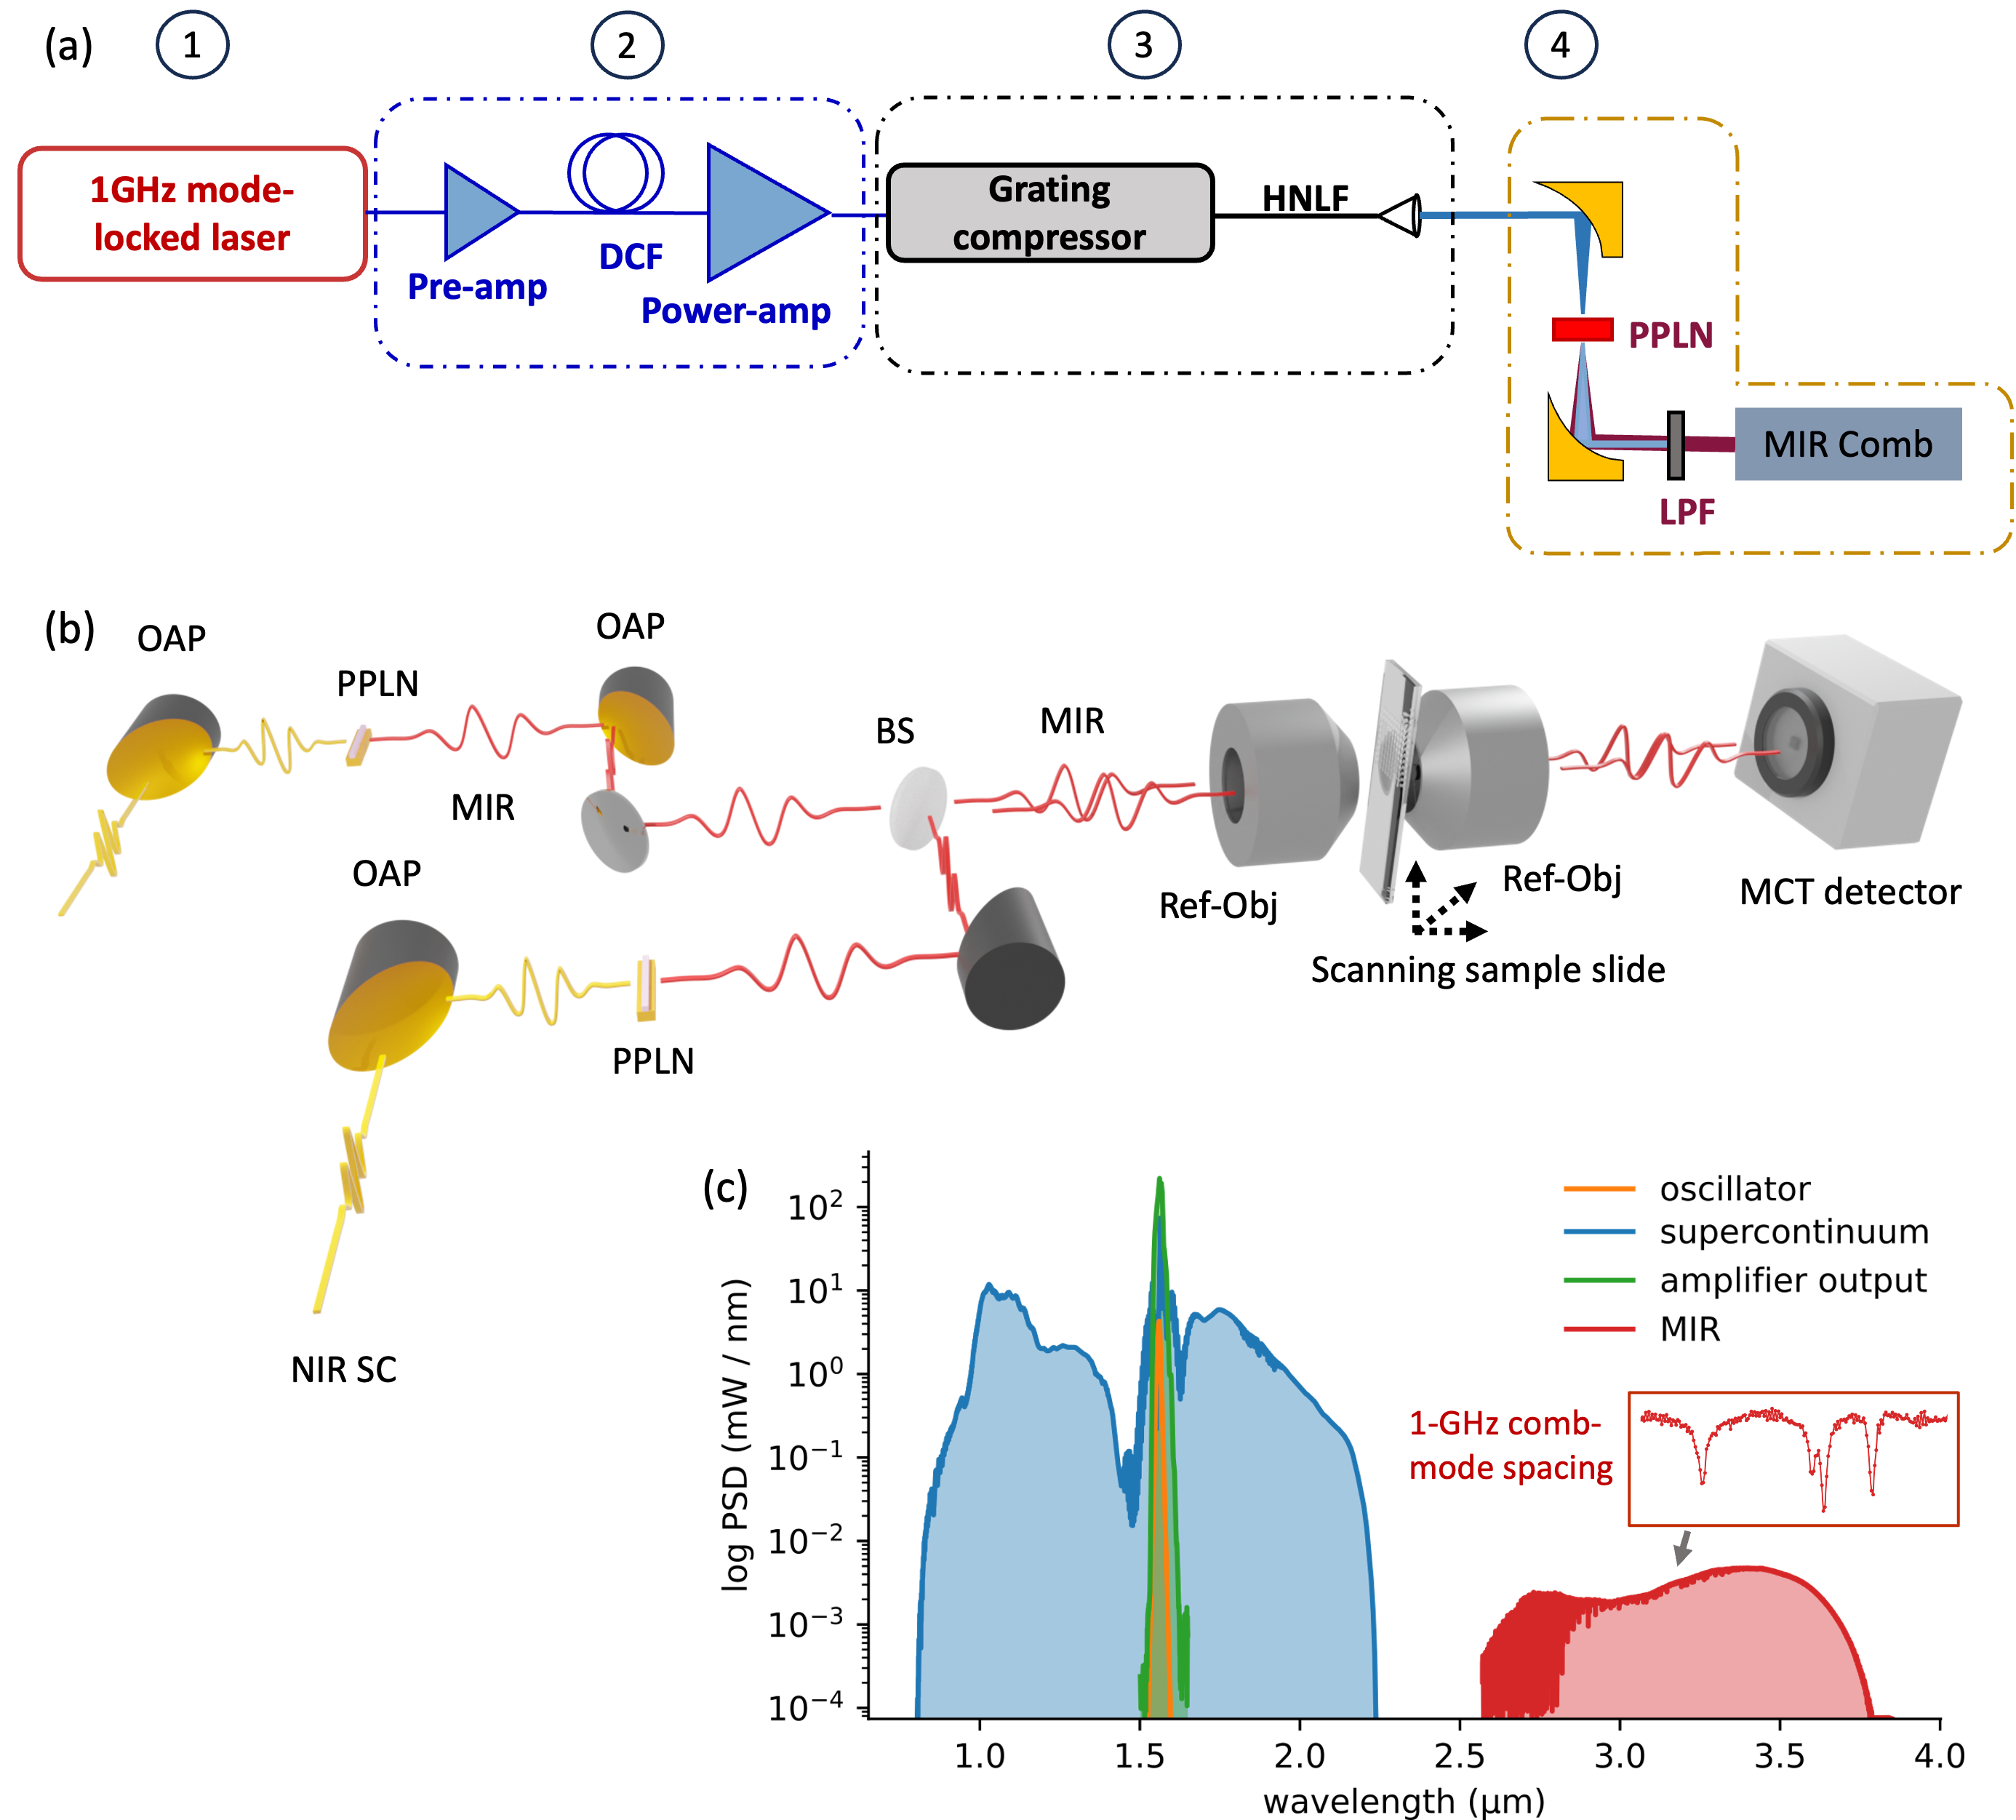
\includegraphics[width=\linewidth]{setup_3D_v3.png}
    \caption{Experimental Setup. Two mid-infrared frequency combs generated through intra-pulse difference frequency generation are passed collinearly through a confocal microscope. Hyperspectral images are collected by raster scanning the sample slide. The transmitted signal is collected and digitized in a high-speed MCT mid-infrared detector and FPGA.}
    \label{fig:setup}
\end{figure}

Two 1-GHz mid-infrared frequency combs are generated and coupled into $\mathrm{InF_3}$ single-mode fiber for delivery to the experiment. The output beam is collimated with a two inch off-axis parabolic mirror, and a reflective confocal microscope with 0.58 NA is used to image the beam onto a glass slide (\mbox{$\sim$3.8 $\mathrm{\mu m}$} pixel size). A set of linear translation stages are used to raster scan the sample. The data is acquired via trigger, with the trigger spacing and scan speed set by the desired spatial sampling interval. The scan speed is limited only by the interferogram acquisition time, which is fundamentally set by the repetition rate of the laser. The transmitted signal is focused onto a high-speed MCT detector, whose AC coupled port is digitized at 1 GS/s using an FPGA (GaGe model \#). The data is streamed concurrently from the card memory into PC RAM for real-time analysis, and such that the card-memory does not limit the data volume. Owing to the fairly high 500 MHz Nyquist frequency, and the placement of all fiber amplifiers in loop for the phase-locks of the two frequency combs, over one thousand interferograms can be directly averaged before phase correction needs to be employed \cite{hebertSelfcorrectedChipbasedDualcomb2017,hebertSelfCorrectionLimitsDualComb2019}.

% ---- move snr analysis to here ----

% -----

To verify the spatial resolution, hyperspectral images are taken of a USAF resolution target composed of SU-8 photoresist patterned onto a 500 $\mathrm{\mu m}$ thick Silicon wafer. Five hundred spectra (39 ms) are averaged at each pixel and apodized to 100 GHz (\mbox{3.3 $\mathrm{cm^{-1}}$}). Point spectra shown in \mbox{Fig. \ref{fig:su8}.(b).} are taken at each pixel to generate the hypercube. The images are generated by integrating a \mbox{$\sim$63 $\mathrm{cm^{-1}}$} window around the peak absorption at \mbox{$\sim$2930 $\mathrm{cm^{-1}}$}. 

% The SU-8 doesn't work too well as a knife-edge, so it's hard to state a spatial resolution that's rigorously calculated.

\begin{figure}[h]
    \centering
    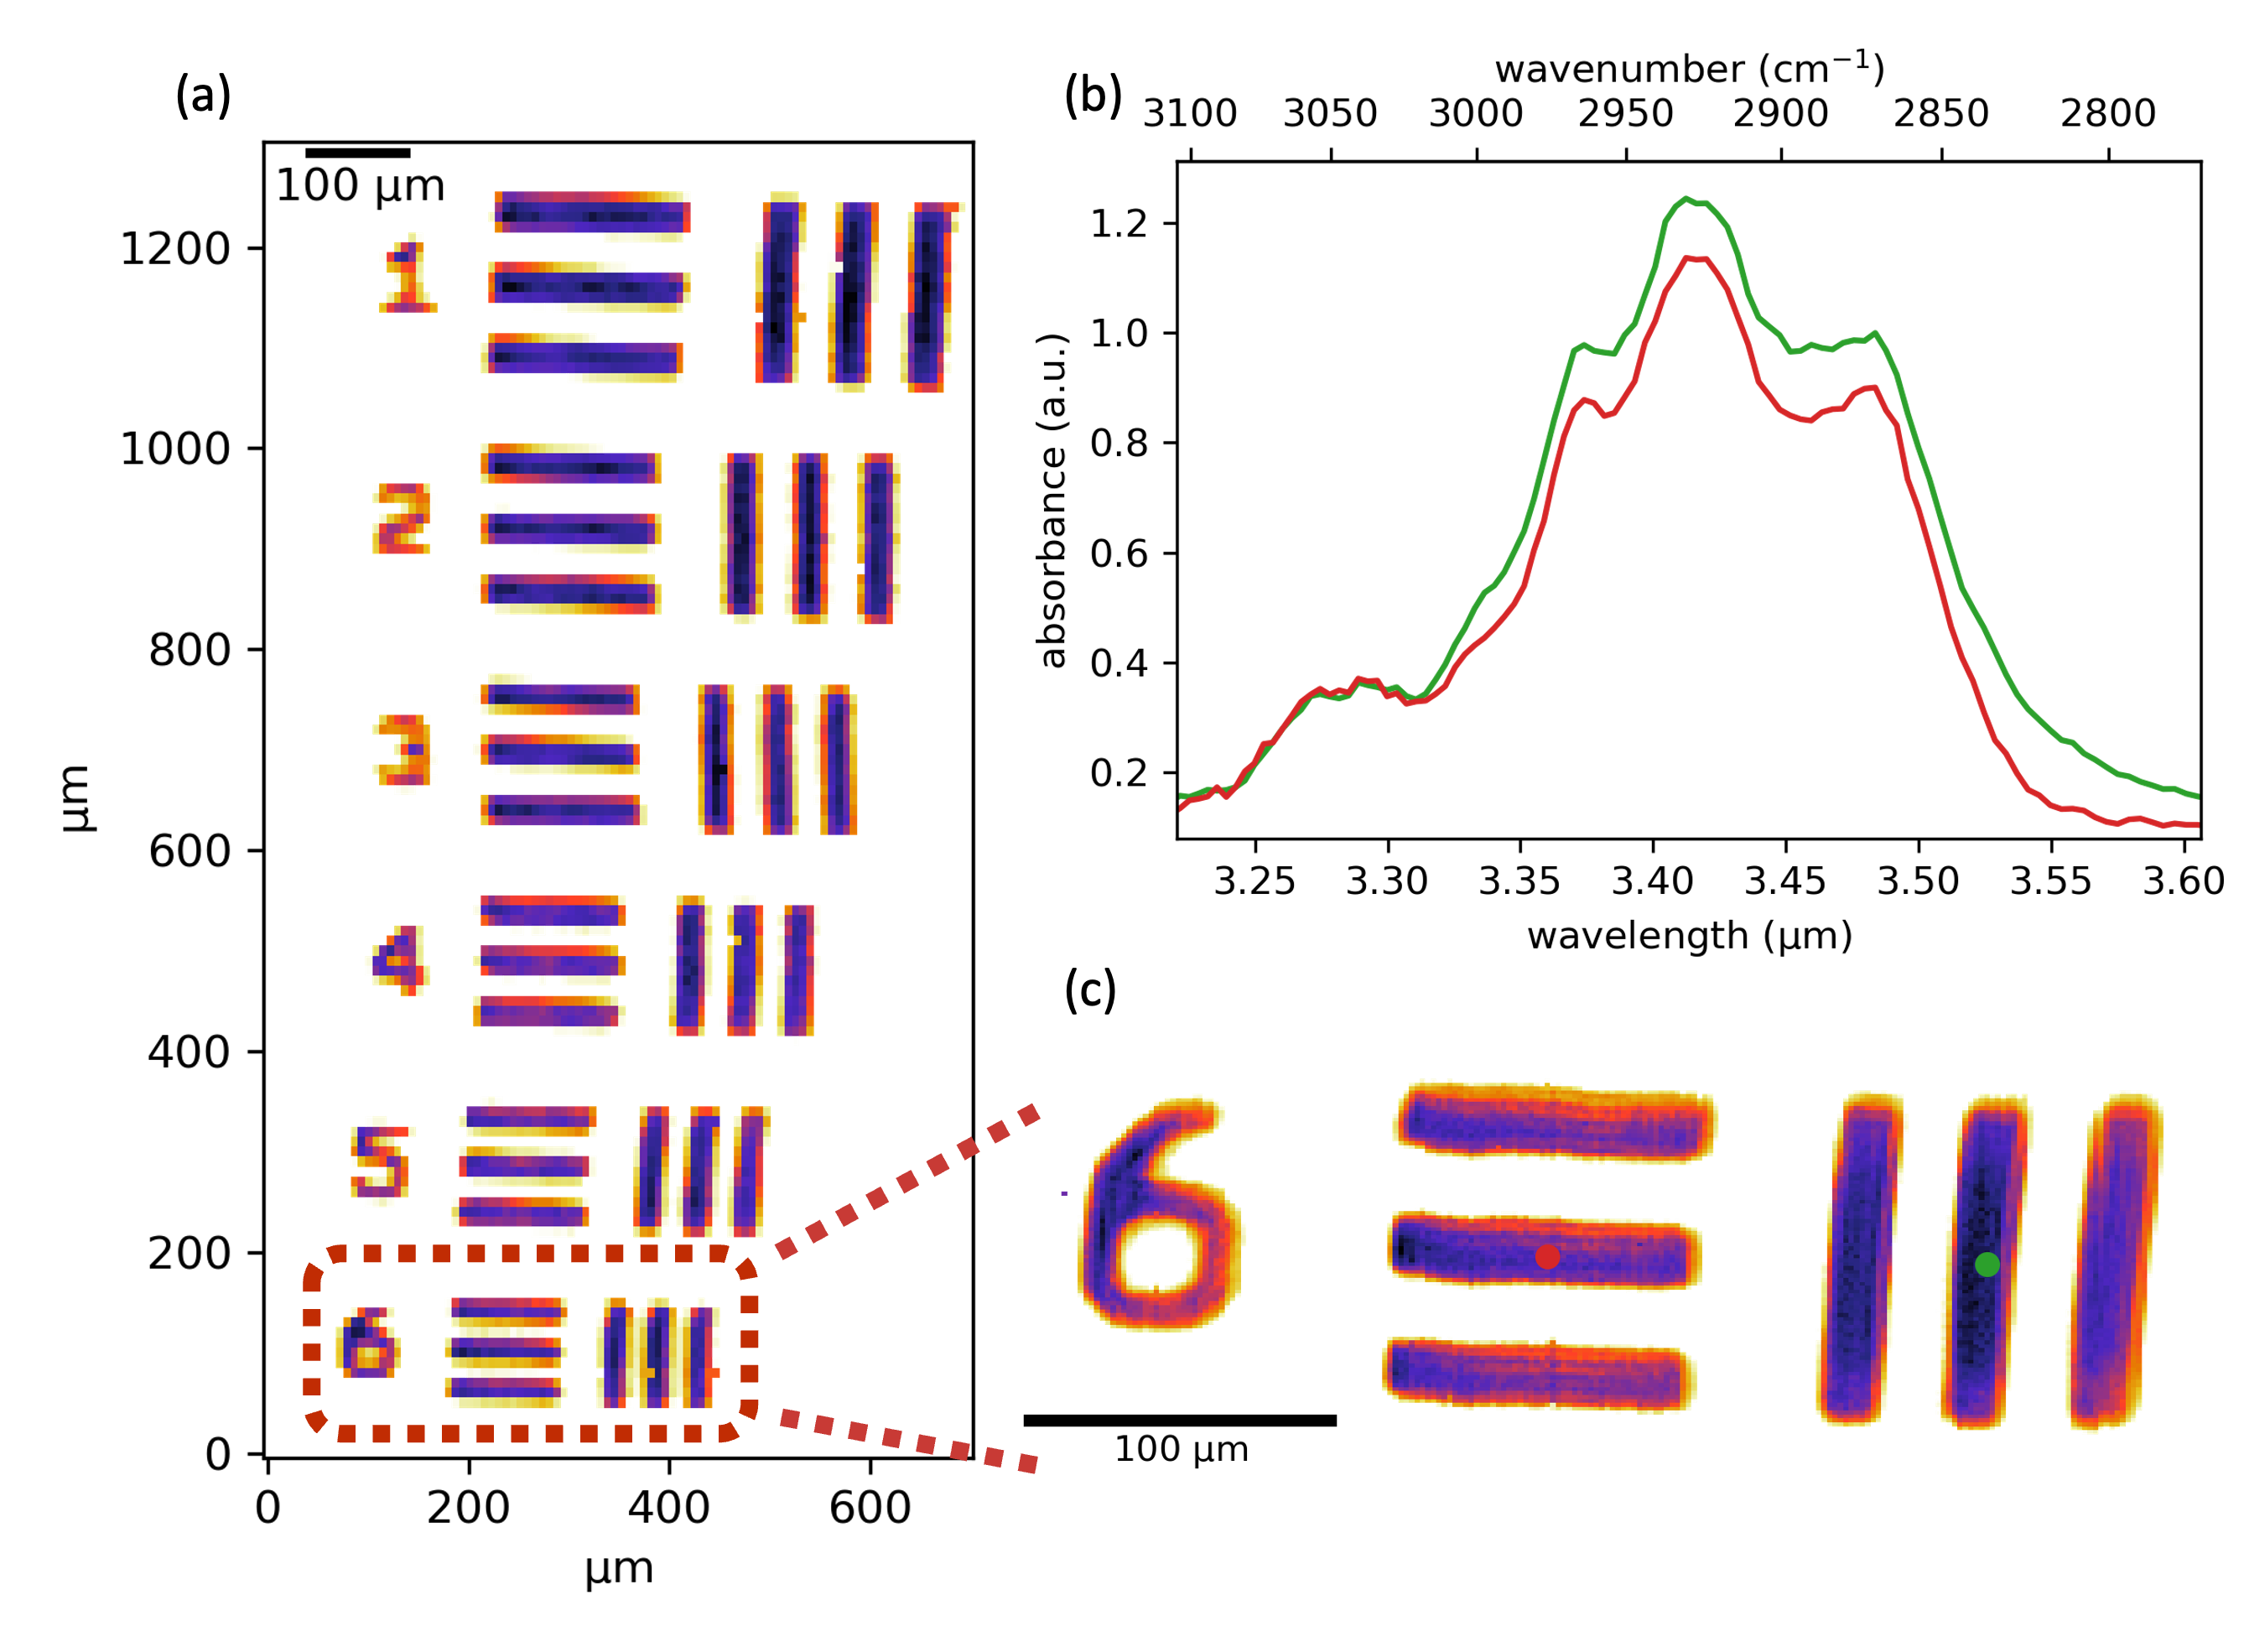
\includegraphics[width=\linewidth]{su8_image.png}
    \caption{Hyperspectral image of SU-8 USAF test pattern on Silicon (a) integrated absorbance around \mbox{2930 $\mathrm{cm^{-1}}$} taken at \mbox{5 $\mathrm{\mu m}$} spatial sampling (b) absorbance curves taken at the red and green points in (c), a finer zoom in of the image in (a) taken at \mbox{1.2 $\mathrm{\mu m}$} spatial sampling.}
    \label{fig:su8}
\end{figure}

For a biologically relevant sample, we image a cross-section of ovarian cancer tissue (\dots add info), where the paraffin wax was removed prior to dual-comb imaging. To validate these results, we compare the results of DCS point scanning microscopy to hyperspectral data taken with a commercial FTIR microscope using a focal plane array (\dots add info). Five hundred spectra are again averaged at each pixel and apodized to \mbox{3.3 $\mathrm{cm^{-1}}$}. Point spectra such as the one shown by the orange curve in \mbox{Fig. \ref{fig:bio}.(b).} are collected at each pixel, with the two C-H anti-symmetric stretch bands visible at 2850 and \mbox{2920 $\mathrm{cm^{-1}}$}. A DCS spectrum taken with a two second averaging time (25,700 averages) is shown by the green curve, and a comparison spectrum taken using a commercial FTIR with \mbox{7.61 $\mathrm{cm^{-1}}$} frequency resolution is shown by the red curve. Apart from a broadening of the peak, good agreement is observed between the DCS and FTIR spectra. The FTIR image was taken prior to the removal of paraffin wax, which accounts for the peak broadening when compared to the spectra taken using DCS. The images are generated by taking a slice through the hypercube at the peak of the \mbox{2920 $\mathrm{cm^{-1}}$} band. A coarse image shown in \mbox{Fig. \ref{fig:bio}.(c).} with \mbox{5 $\mathrm{\mu m}$} sampling is taken of the entire core. A zoom-in of the sample is shown in \mbox{Fig. \ref{fig:bio}.(a).}, taken at \mbox{1.2 $\mathrm{\mu m}$} sampling, which is approximately the Nyquist sampling limit of the microscope. The image shows generally good agreement with the corresponding image in \mbox{Fig. \ref{fig:bio}.(d).} taken using FTIR. We note that the dim vertical line scans in the DCS image are attributed to the limited \mbox{$\sim$1.5 $\mathrm{\mu m}$} repeatibility of the translation stages (Thorlabs Z825B).

% In addition to the spectral comparison, spatial comparison is also good ...

\begin{figure}[h]
    \centering
    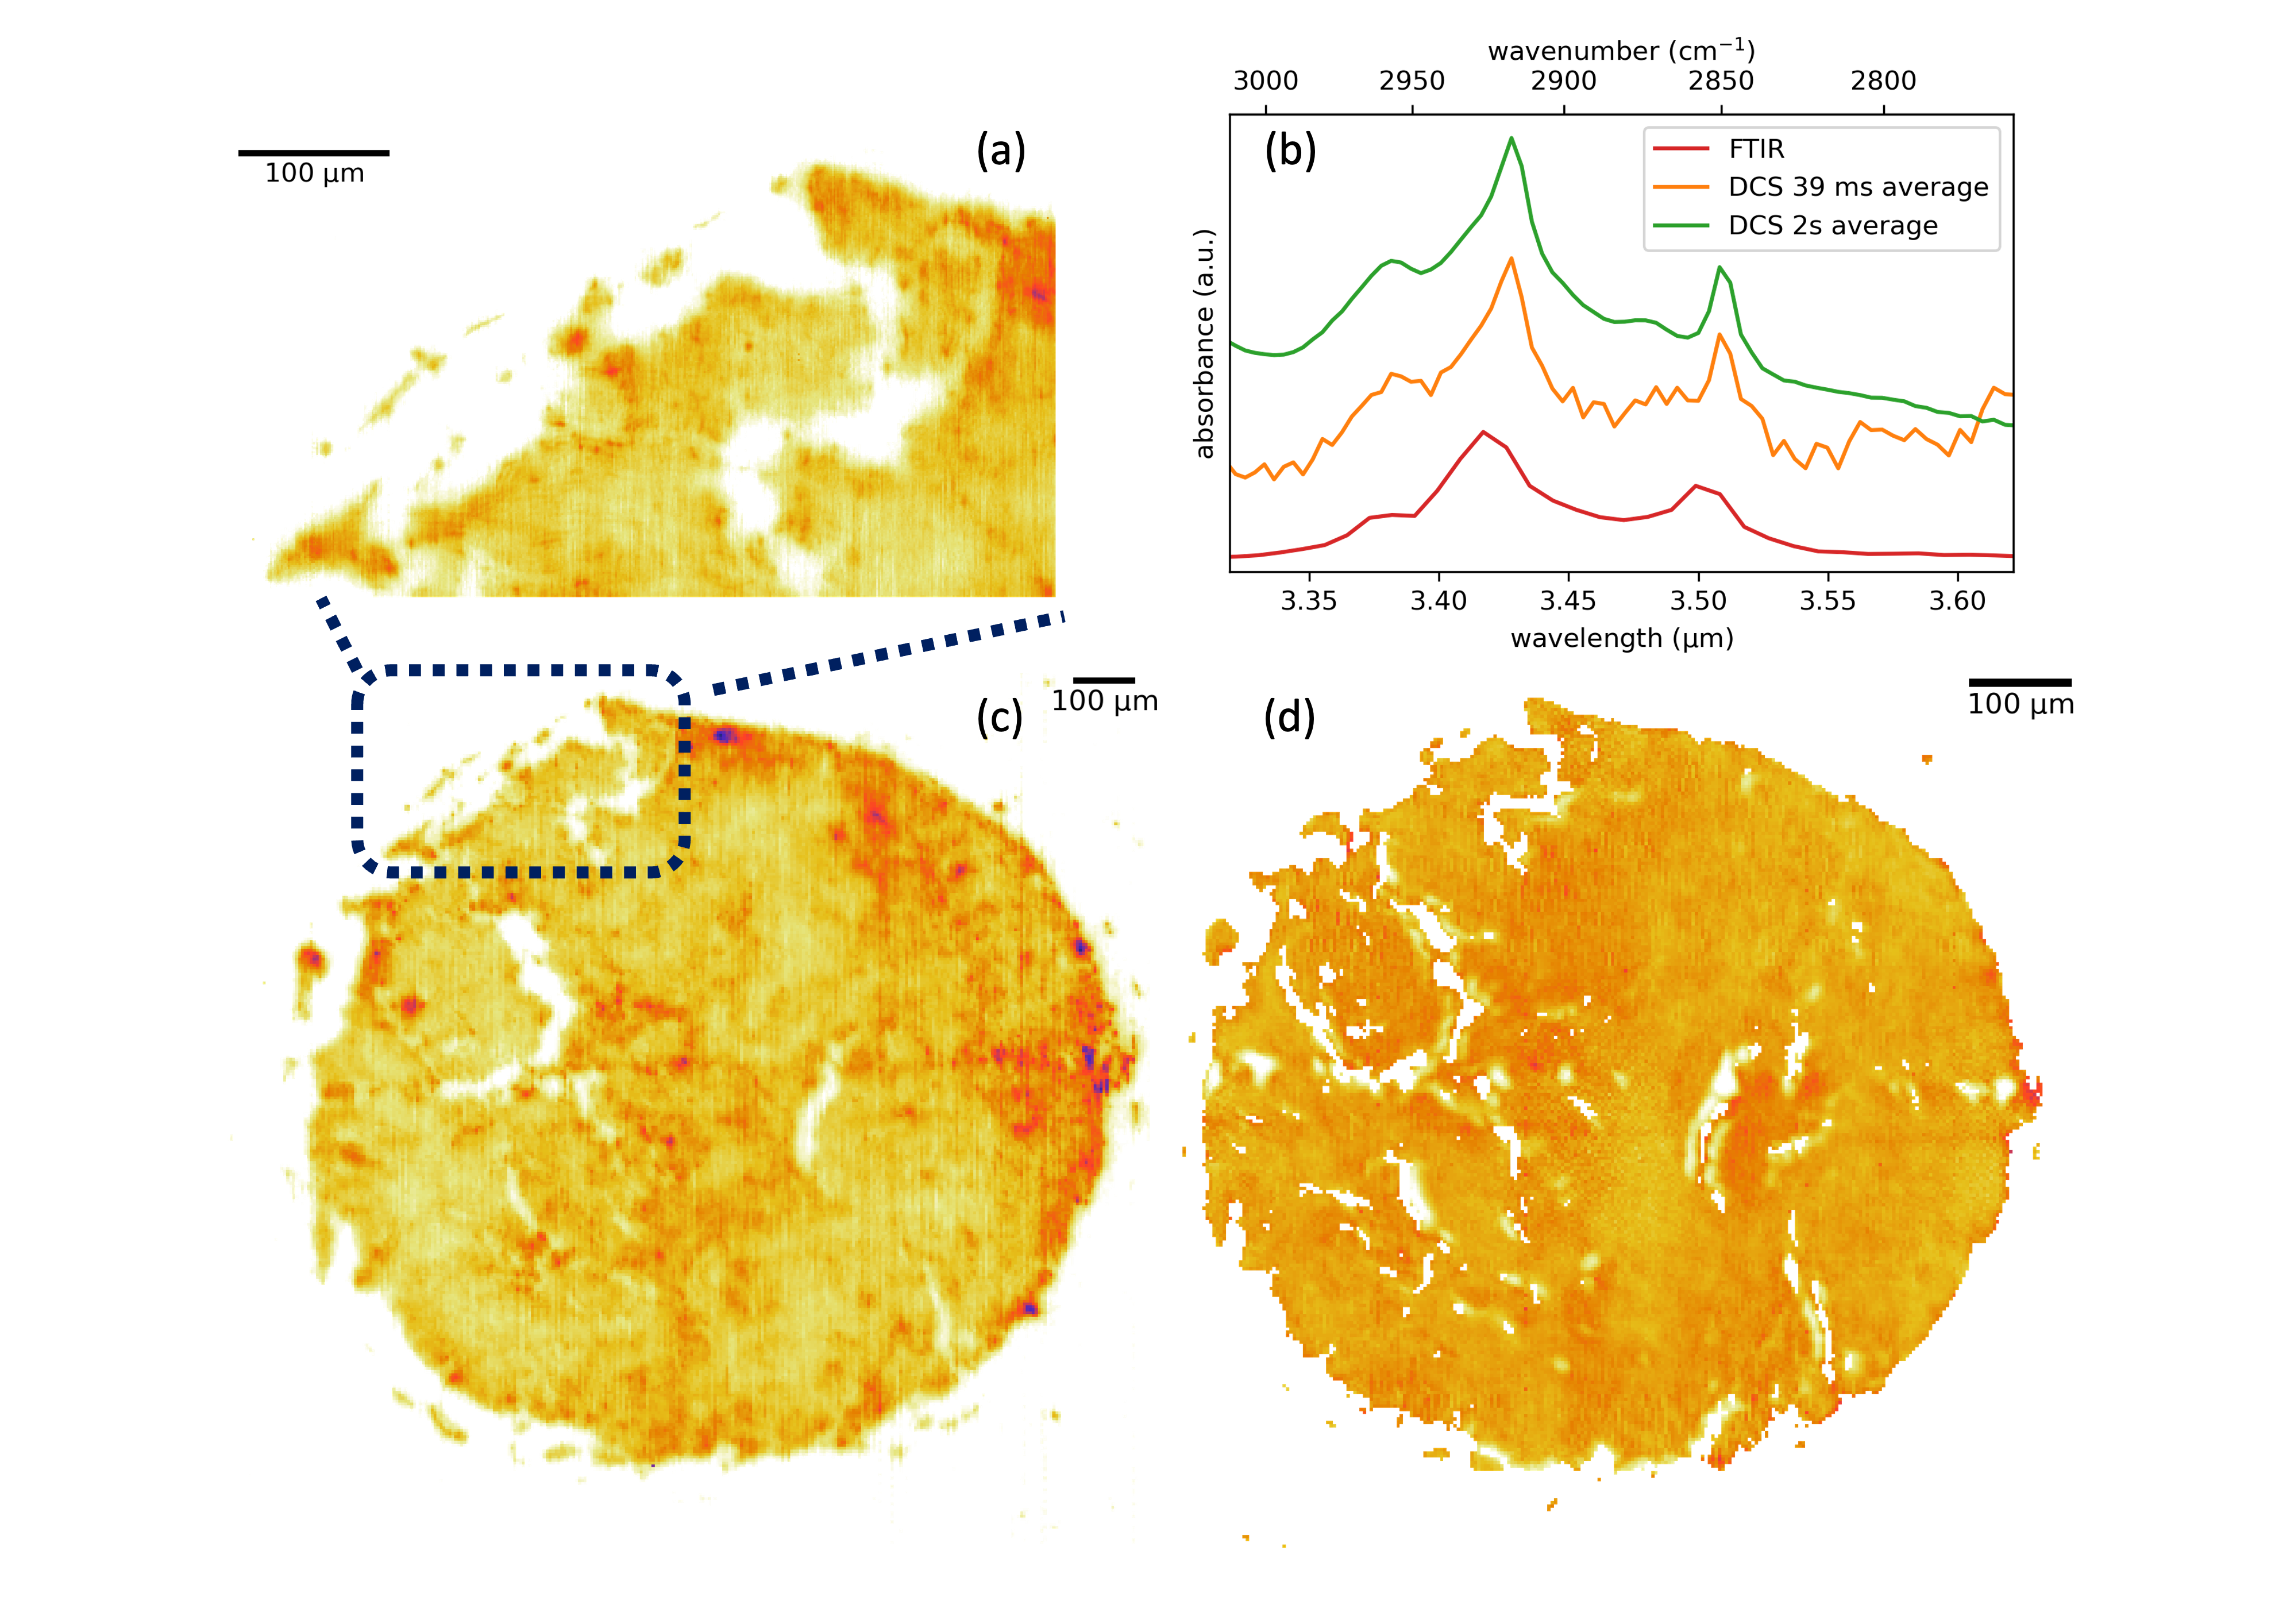
\includegraphics[width=\linewidth]{bio_image_w_FTIR_comparison.png}
    \caption{Hyperspectral image of ovarian cancer tissue (a) absorbance at \mbox{2920 $\mathrm{cm^{-1}}$} taken at \mbox{1.2 $\mathrm{\mu m}$} sampling (b) Absorbance curves taken on cancer tissue with two second average in green, 39 ms average in orange, and with a commercial FTIR in red (c) zoom out of (a) to include absorbance image of the whole core at \mbox{2920 $\mathrm{cm^{-1}}$} taken with \mbox{5 $\mathrm{\mu m}$} spatial sampling (d) equivalent image to (c) but taken using a commercial FTIR microscope using a focal plane array.}
    \label{fig:bio}
\end{figure}

\section{Discussion}
The final determination of imaging speed is given by the time needed to reach sufficient SNR at each pixel. Specifically for DCS microscopy, the target SNR and frequency resolution sets the pixel dwell time. In DCS, the absorbance noise $\sigma$ scales with the frequency resolution and number of averaged spectra $N_{avg}$ according to \cite{newburySensitivityCoherentDualcomb2010}: 
% 
\begin{align}
    \sigma \propto \frac{N}{\sqrt{N_{avg}}}
    \label{eq:snr}
\end{align}
% 
where $N$ is the number of frequency bins. This scaling rule is shown in \mbox{Fig. \ref{fig:snr_analysis}.(c-d).}, where it is observed to match the experimentally measured absorbance noise. 

% The two-variable map in  \mbox{Fig. \ref{fig:snr_analysis}.(d).} should apply more generally to any DCS point scanning microscopy, but with the time axis scaled accordingly to the repetition rate as $\propto 1 / f_r^2$. 

\begin{figure}[h]
    \centering
    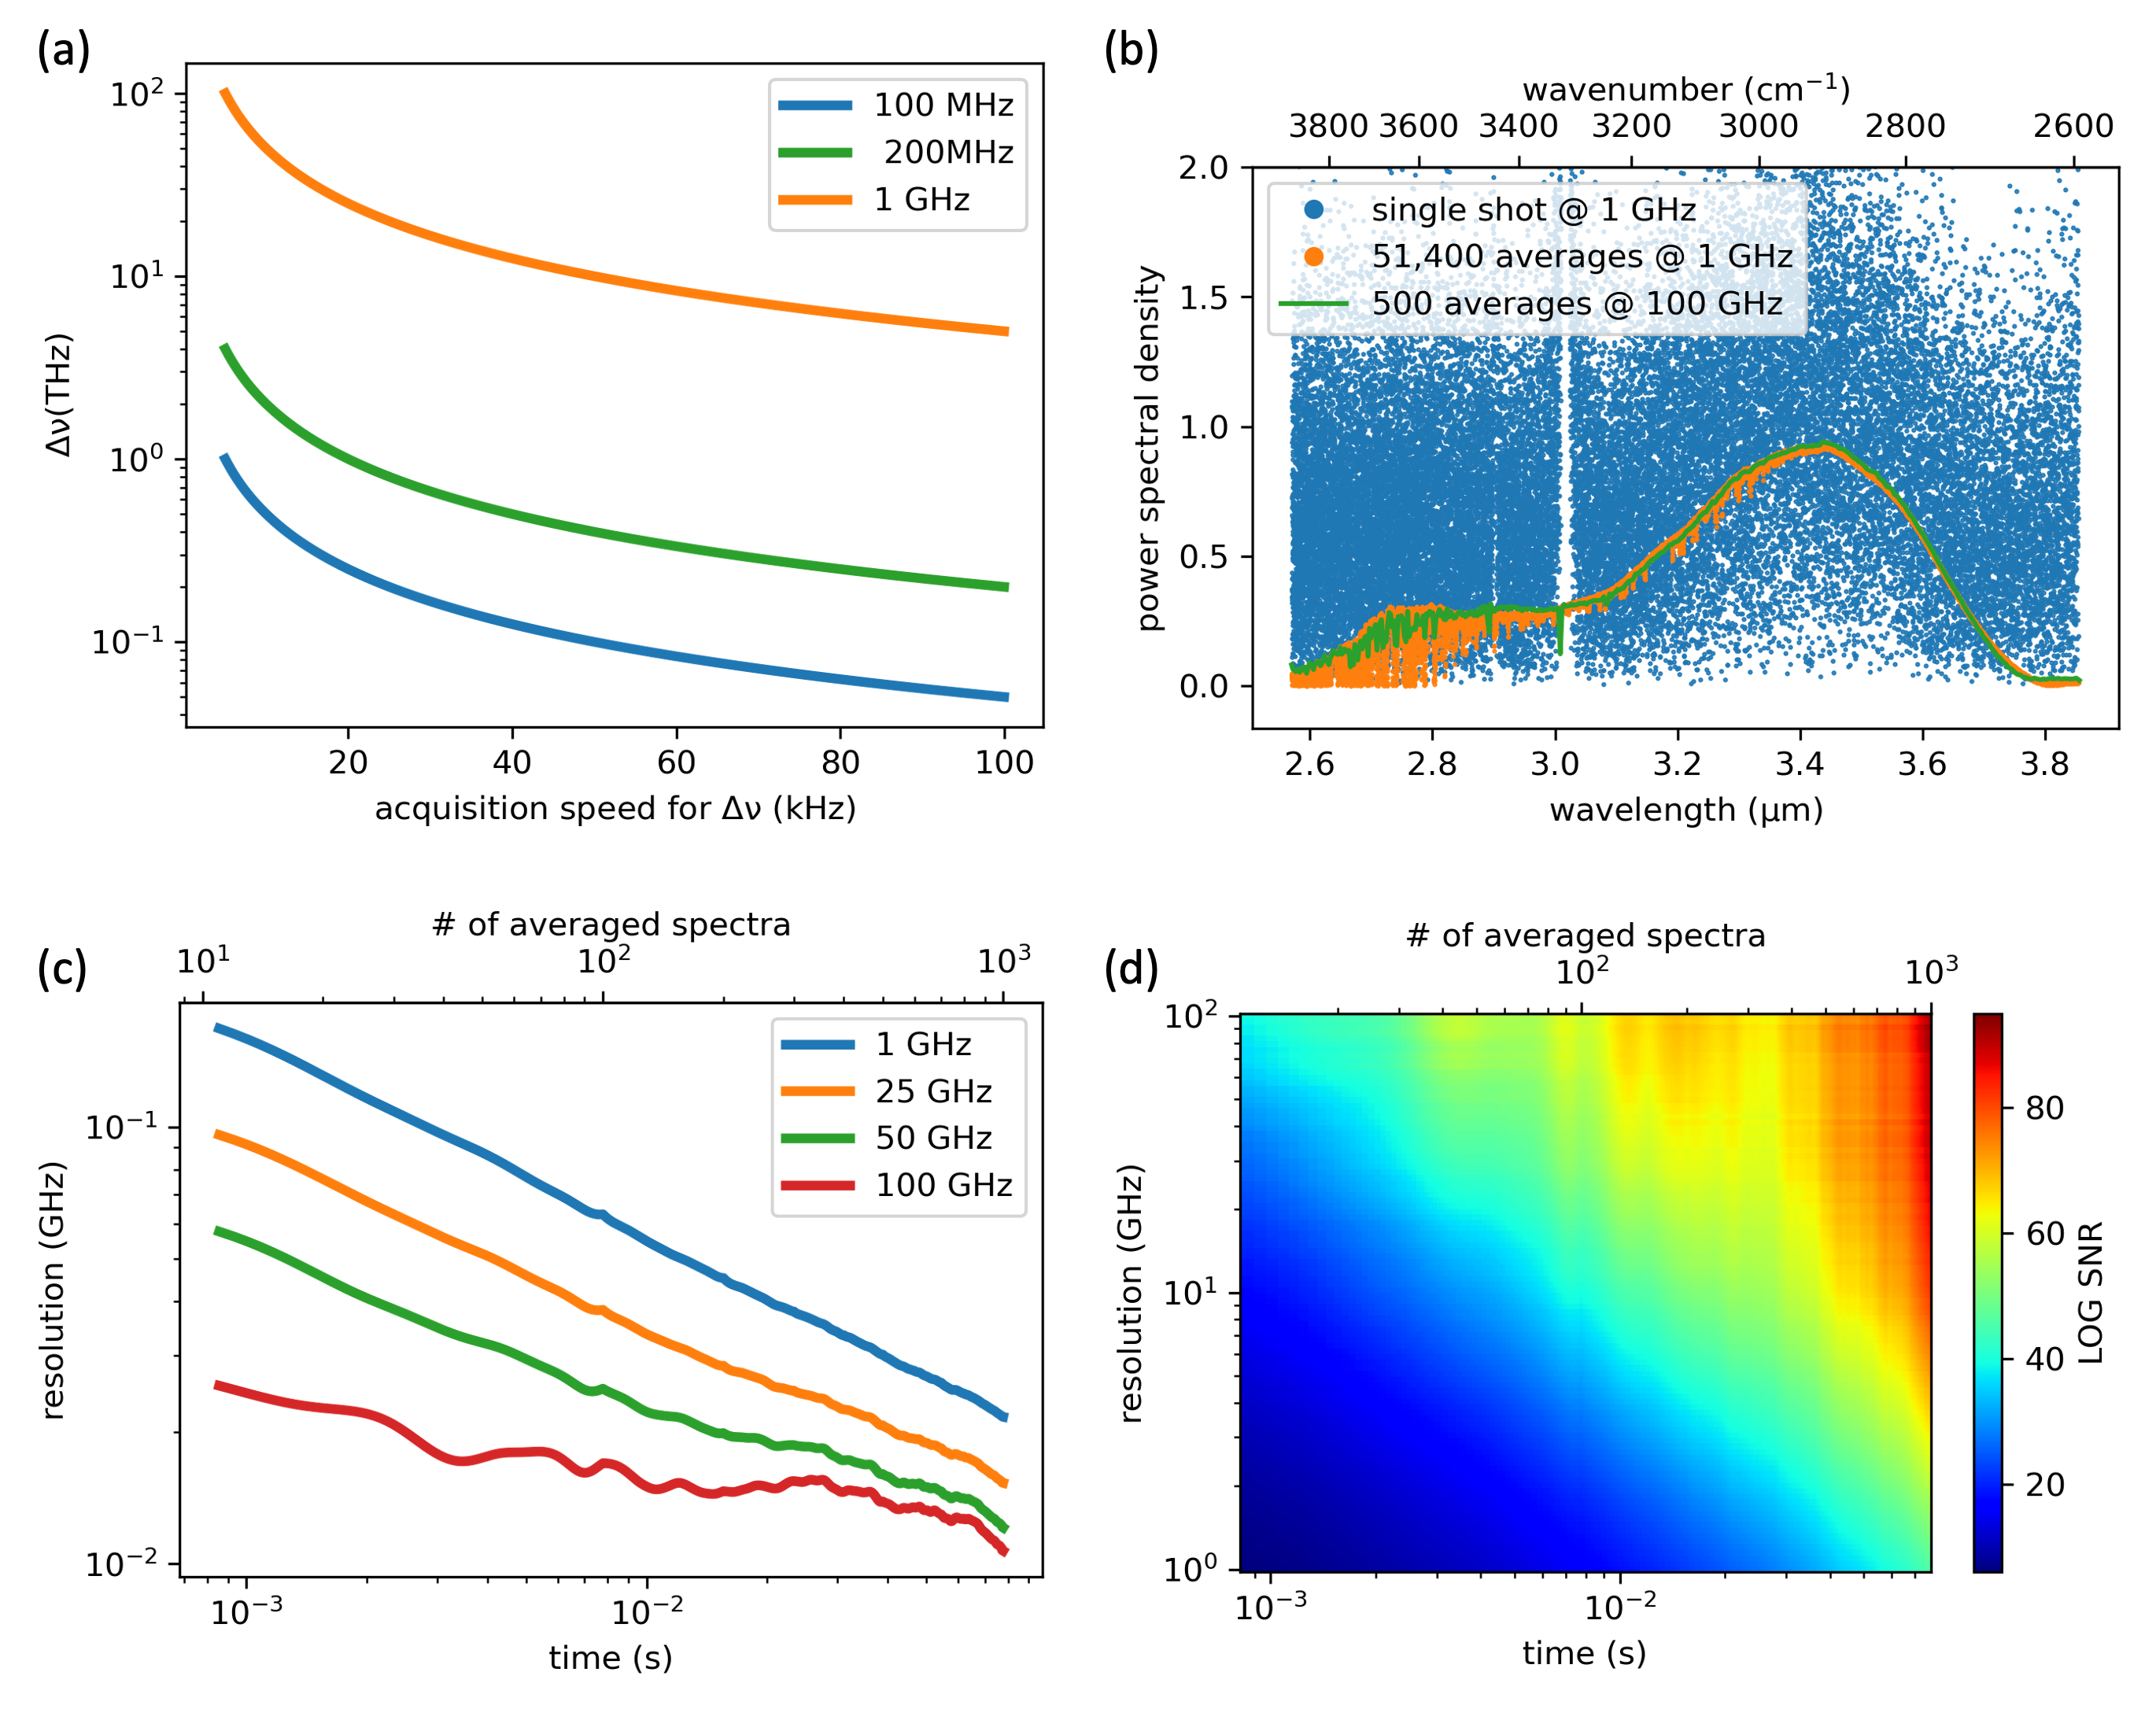
\includegraphics[width=\linewidth]{snr_analysis.png}
    \caption{Summary of DCS Imaging Speed. (a) The size of the optical Nyquist window plotted against acquisition speed (\mbox{$\Delta f_r$}) for different repetition rates. (b) DCS spectrum taken at different averaging times and frequency resolution/apodization windows. (c) The spectra's SNR follow the scaling of \mbox{Eq.\ref{eq:snr}}, with an example of the 2D parameter space (d) mapped out for the 1-GHz system.}
    \label{fig:snr_analysis}
\end{figure}

Shown in \mbox{Fig. \ref{fig:snr_analysis}.(a).}, a baseline for 1 GHz DCS is that a 1000 $\mathrm{cm^{-1}}$ Nyquist window can be covered with \mbox{$\sim$17 kHz} spectra acquisition speed. In \mbox{Fig. \ref{fig:snr_analysis}.(b).}, a single-shot spectrum (77 $\mathrm{\mu s}$) at 1 GHz resolution has low signal to noise, but can be averaged to high SNR in two seconds (>25,000 spectra). However, a high SNR can be achieved in \mbox{$\sim$39 ms} at 500 averages if the interferograms are apodized to 100 GHz (\mbox{$\sim$3.33 $\mathrm{cm^{-1}}$}), which is a more appropriate sampling interval for the given absorption features. The SNR as a function of averaging time and frequency resolution is shown in \mbox{Fig. \ref{fig:snr_analysis}.(c-d).}; the absorbance noise always averages down according to $1/\sqrt{N_{avg}}$, but with coarser resolution resulting in a directly proportional overall noise reduction. 

All time scales change with the repetition rate as $\propto 1 / f_r^2$. Consequently, the two-variable map in  \mbox{Fig. \ref{fig:snr_analysis}.(d).} should apply more generally to DCS point scanning microscopy with lower and higher $f_r$, but with the time-axis scaled accordingly. As an example, well established 100 MHz mid-infrared DCS \cite{lindMidInfraredFrequencyComb2020,timmersMolecularFingerprintingBright2018} would reach the same SNR at 3.9 s per pixel extending the overall experiment time to over a day, \cite{timmersHyperspectralMicroscopyBroadband2019}, while 10 GHz DCS would reach the SNR in 390 $\mathrm{\mu s}$ reducing the overall experiment time from the several hours in this experiment down to minutes.

\section{Conclusion}

% pass v1 at a conclusion
In conclusion, we demonstrate a high rep-rate and broadband DCS microscope covering over $1000 \; \mathrm{cm^{-1}}$ in the mid-infrared. The results are used to create a performance map for future DCS applications in microscopy. At a 1 GHz rep-rate, DCS brings the point scanning system's overall experiment time to comparable numbers as FTIR microscopes that buy their speed from employing focal plane arrays, with acquisition times of a few hours for a 512x512 image after averaging at each pixel. The DCS point scanning system offers a frequency axis calibrated to an uncertainty of the measured rep-rate around $\mathrm{10^{-11}}$, and whose resolution can be chosen down to the comb mode-spacing. The point scanning system also offers greater flexibility, as it leaves open the possibility for compressed sensing. Importantly, compression could be performed not only on spatial sampling, but also spectrally by employing a time programmmable frequency comb to implement a real-time apodization, for example \cite{tourigny-planteApodizationDualcombSpectroscopy2020,kawaiCompressiveDualcombSpectroscopy2021,caldwellTimeprogrammableFrequencyComb2022}. From known work, compressively sampling the time domain interferogram can artifically pushing the system past the 10 GHz mode-spacing regime using digital locking electronics alone, and introduce accelerated imaging times reduced by factors over a hundred. We anticipate that further work in combining advanced platforms utilized by the gas-sensing and imaging community can realize a compact and robust solution to broad-band and high speed vibrational imaging. 

% ending statement to add to above paragraph:
% We anticipate that further work in combining the advanced platforms utilized by the gas-sensing and imaging community can realize a compact and robust solution to broad-band and high speed vibrational imaging. 

\bibliography{references}

\end{document}
